% Part: sets-functions-relations
% Chapter: relations
% Section: trees

\documentclass[../../../include/open-logic-section]{subfiles}

\begin{document}

\olfileid{sfr}{rel}{tre}
\olsection{درخت (Trees)}

جزوی ترتیب (partial order) دی اک خاص قسم، جیہڑی منطق دے سارے حصیاں وچ
اہم کم کردی اے، \emph{درخت} (tree) اے۔ محدود درخت (finite trees) منطق
دے ابتدائی حصیاں وچ آؤندے نیں: مثال لئی، !!{formula}s نوں اوہناں دے
نحوی درخت (syntax tree) وچ ٹوٹن دے لحاظ نال سمجھیا جا سکدا اے، جد کہ
!!{derivation}s (derivations) کئی !!{derivation} نظاماں (derivation
systems) وچ وی محدود درختاں دی صورت اختیار کردے نیں۔
%
لامتناہی درخت (infinite trees) قضیاتی منطق (propositional logic) تے پہلے
درجے دی منطق (first-order logic) دے تمامیت دے قضیاں (completeness
theorems) دے ثبوتاں وچ ای آ جاندے نیں، تے ریاضیاتی منطق (mathematical
logic) وچ تھاں تھاں ورتے جاندے نیں۔

سیٹ نظریاتی تصور (set-theoretic concept) دے طور تے درخت، گراف نظریے
(graph theory) دے درخت نال گہرا تعلق رکھدا اے۔ اک (محدود) درخت دی
تصویر ایہ اے:

\begin{center}
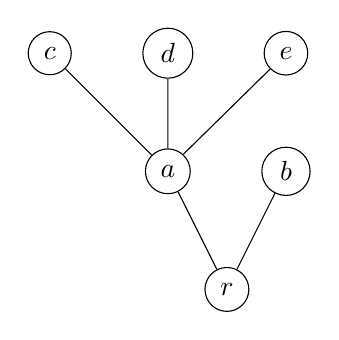
\begin{tikzpicture}[nodes={draw, circle}, -]
\node{$r$} [grow'=up]
    child { node {$a$} 
        child { node {$c$} }
        child { node {$d$} }
        child { node {$e$} }
    }
    child { node {$b$} };
\end{tikzpicture}
\end{center}

سب توں تھلّے والی گرہ (node)~$r$ جڑ (root) اے۔ $r$ توں ہٹ کے ہر گرہ
دی عین تھلّے صرف اک والد گرہ (parent node) ہوندی اے۔ اسی گرہ~$x$ دا
گرہ~$y$ نال اوہ تعلق، جیہڑا اُدوں ہووے جدوں $y$ تیکر~$x$ توں کناریاں
(edges) دے نال نال اُتّے نوں جا کے پہنچ سکّیے، ایویں سمجھ سکدے آں کہ
$x$، گرہ~$y$ دا \emph{پُرکھ} (ancestor) اے۔

درخت وچ پُرکھ ہون دا تعلق سخت جزوی ترتیب (strict partial order) اے۔ ایہ
گل سیٹ نظریے والی تعریف دا محرک اے۔ اوہ تعریف دسن لئی سانوں دو تصور
چاہیدے نیں۔ کسے سیٹ~$A$ وچ، جیہنوں~$\le$ نال جزوی ترتیب دتی گئی ہووے،
\emph{سب توں چھوٹا عنصر} (least element) اوہ !!a{element} $x \in A$
اے جیہدے لئی ہر $y \in A$ اُتے~$x \le y$ ہووے۔ اک سیٹ، تعلق~$\le$ دے
لحاظ نال \emph{حُسنِ ترتیب والا} (well-ordered) ہوندا اے جے اوہدے ہر
غیر خالی ذیلی سیٹ دا سب توں چھوٹا عنصر ہووے۔

\begin{defn}[درخت (Tree)]
اک \emph{درخت} (tree) جوڑا $T = \tuple{A, \le}$ اے جیہدے وچ $A$ اک
سیٹ تے $\le$، سیٹ~$A$ اُتے جزوی ترتیب (partial order) ہووے، تے اک
اکلوتا سب توں چھوٹا عنصر (unique least element) $r \in A$ (جیہنوں
\emph{جڑ} (root) آکھدے نیں) ہووے، ایس طرح کہ ہر $x \in A$ لئی، سیٹ
$\Setabs{y}{y \le x}$، تعلق~$\le$ دے لحاظ نال حُسنِ ترتیب والا
(well-ordered) ہووے۔
\end{defn}

\begin{defn}[جانشین (Successors)]
من لو کہ $T = \tuple{A, \le}$ اک درخت اے۔ جے $x,y \in A$، $x < y$،
تے کوئی وی $z \in A$ ایہو جیہا نہ ہووے کہ $x < z < y$، تاں اسی آکھدے
آں کہ $y$، گرہ~$x$ دا \emph{جانشین} (successor) اے۔
\end{defn}

گرہ $x \in A$ دے جانشین اوہدے \emph{بچے} (children) وی آکھلاندے نیں۔
جے $y$، گرہ~$x$ دا جانشین اے، تاں اسی $x$ نوں گرہ~$y$ دا
\emph{پیشرو} (predecessor) یا \emph{والد گرہ} (parent) آکھدے آں۔

\begin{prop}
جے $\tuple{A,\le}$ اک درخت اے، تاں جڑ توں ہٹ کے ہر $x \in A$ دا ودھ
توں ودھ اک پیشرو ہوندا اے۔
\end{prop}

\begin{proof}
  من لو کہ $y_1 < x$ تے $y_2 < x$ تے $y_1 \neq y_2$۔ تاں $\{y_1,
  y_2\} \subseteq \Setabs{z}{z<x}$۔ کیوں جے $\Setabs{z}{z<x}$،
  تعلق~$\le$ دے لحاظ نال حُسنِ ترتیب والا اے، اوہدے ذیلی سیٹ
  $\{y_1, y_2\}$ دا سب توں چھوٹا عنصر اے، جیہڑا صاف طور تے یا $y_1$
  یا~$y_2$ ہونا چاہیدا اے۔ سو یا $y_1 \le y_2$ یا $y_2 \le y_1$۔ اسی
  منّیا سی کہ $y_1 \neq y_2$، سو اصل وچ یا $y_1 < y_2$ یا $y_2 < y_1$۔
  کیوں جے اسی منّیا سی کہ $y_1 < x$ تے $y_2 < x$، ایس لئی نالے یا
  $y_1 < y_2 < x$ یا $y_2 < y_1 < x$۔ سو $y_1$ تے $y_2$ دونویں،
  گرہ~$x$ دے پیشرو نہیں ہو سکدے۔
\end{proof}

\begin{defn}
درخت $T = \tuple{A, \le}$ \emph{لامتناہی} (infinite) آکھلاندا اے جے
$A$ لامتناہی سیٹ ہووے، تے نہیں تاں \emph{محدود} (finite)۔ جے $T$ ایہو
جیہا ہووے کہ ہر $x \in A$ دے صرف محدود گنتی وچ جانشین ہون، تاں اسی
آکھدے آں کہ $T$ \emph{ہر راس دے محدود جانشیناں والا} (finitely
branching) اے۔
\end{defn}

\begin{defn}[شاخاں (Branches)]
دتے ہوئے درخت $T = \tuple{A, \le}$ دی \emph{شاخ} (branch)، $T$ وچ اک
ہور نہ ودھ سکن والی زنجیر (maximal chain) اے، یعنی $T$ وچ اک سیٹ
$B \subseteq A$ جیہڑا ایہو جیہا ہووے کہ ہر $x, y \in B$ لئی یا
$x \le y$ یا $y \le x$، تے ہر $z \in A \setminus B$ لئی کوئی
$u \in B$ ایہو جیہا موجود ہووے کہ نہ $z \le u$ تے نہ $u \le z$۔
ماخذ وچ ایتھے غیر متعین X دی تھاں درخت دا حامل سیٹ A ورتیا گیا اے
(PNBREL-001)۔
%
اسی $[T]$ نال $T$ دیاں ساریاں شاخاں دا سیٹ ظاہر کردے آں۔
\end{defn}

\begin{ex}
ہر راس دے محدود جانشیناں والے (finitely branching) درخت دی اک مشہور
مثال، $0$ تے~$1$ دے محدود سلسلیاں دا \emph{لامتناہی دو شاخی درخت}
(infinite binary tree) اے، جیہنوں کدی $\{0,1\}^*$ یا~$\Bin^*$ نال
ظاہر کردے نیں، تے ودھاؤ دے تعلق (extension relation) $\sqsubseteq$
نال ترتیب دیندے نیں (مثلاً $101 \sqsubseteq 101101$)۔ کیوں جے کوئی وی
دو علامتی لڑی (binary string) آخر اُتے $0$ یا $1$ لا کے ہمیشہ ودھائی
جا سکدی اے، ایس درخت وچ لامتناہی عنصر نیں: ہر عنصر~$s$ دے عین دو
جانشین، $s0$ تے~$s1$، نیں۔ اوہدی جڑ خالی سلسلہ (empty sequence)
$\emptyseq$ اے۔
\end{ex}

\begin{ex}
تھوڑا ہور عام طور تے، قدرتی عدداں دے محدود سلسلیاں دا سیٹ~$\Nat^*$،
ودھاؤ دے تعلق~$\sqsubseteq$ نال، وی اک درخت اے۔ صاف ظاہر اے کہ ایہ ہر
راس دے محدود جانشیناں والا (finitely branching) نہیں: ہر $s \in \Nat^*$ دے لامتناہی
جانشین~$sn$ نیں، ہر $n \in \Nat$ لئی اک۔ ہر $A \subseteq \Nat^*$
جیہڑا~$\sqsubseteq$ دے تحت بند ہووے، $\Nat^*$ دا \emph{ذیلی درخت}
(subtree) اے۔
(یعنی $A$ ایہو جیہا اے کہ جے $s \in A$ تے $s' \sqsubseteq s$، تاں
$s' \in A$ وی۔) سارے محدود درخت $\Nat^*$ دے محدود ذیلی درختاں دے طور
تے ظاہر کیتے جا سکدے نیں۔
\end{ex}

\begin{prop}[K\H{o}nig دا معاون قضیہ (König's lemma)]
جے $T = \tuple{A,\le}$، ہر راس دے محدود جانشیناں والا (finitely
branching) لامتناہی درخت اے،
تاں $T$ دی اک لامتناہی شاخ اے۔
\end{prop}

K\H{o}nig دے معاون قضیے دی اک خاص صورت، جیہڑی قابلِ حسابیت دے نظریے
وچ بہت ورتی جاندی اے تے \emph{K\H{o}nig دا کمزور معاون قضیہ} (weak
König's lemma) آکھلاندی اے، ایہ اے: $\{0,1\}^*$ دے ہر لامتناہی ذیلی
درخت دی اک لامتناہی شاخ اے۔

\end{document}
